\chapter{Speed}

\section*{LEARNING OUTCOMES}
{
\begin{center}
\fcolorbox{black}{shadecolor}{%

    \parbox{0.95\textwidth}
    {%
        \small
        {
        \begin{itemize}
            \item Describe the concept of rest and motion to the students.
            \item Describe speed and acceleration as the physical quantities to quantify the motion of an object.
            \item Describe different instruments used to measure speed.
        \end{itemize}
        }
    }%
}
\end{center}
}

\section*{DEMONSTRATIONS}
\section*{Speedometer}

To build a speedometer, you will need:

\begin{table}[H]
    \centering
    \begin{tabular}{|c|l|c|}\hline
    1   &   IR Transmitter          &   2\\\hline
    2   &   IR sensors              &   2\\\hline
    3   &   470 $\Omega$ resistors  &   2\\\hline
    4   &   Box (for assembling the speedometer)     &   1\\\hline
    5   &   Arduino UNO             &   1\\\hline
    6   &   Connecting wires        &   -\\\hline
    \end{tabular}
\end{table}

\subsection*{Connections}
\begin{enumerate}[leftmargin=*]
    \item Flip the box so that the open side is facing downwards. On any of its walls, cut an opening large enough for a small object (ping-pong, toy car etc.) to pass through. On the opposite wall, cut a similar opening so that a path is created for the object.
    \item Fix the Arduino microcontroller on the top of the box. 
    \item Connect the positive and ground terminals of the IR sensors to the 5V and GND terminals of Arduino. 
    \item Connect the OUT pin of the IR sensors to A3 and A4 pin of Arduino. 
    \item Connect each of the anodes of the IR transmitters to a 470 $\Omega$ resistor. Connect the free terminal of the resistors to the 5V pin and the cathodes of the LEDs to GND of Arduino.
    \item Fix an IR LED and an IR sensor on each of the opposite ends of the opening such that they are facing each other.
\end{enumerate}
The circuit diagram of speedometer shows how these components are to be connected:
	\begin{figure}[H]
	\centering 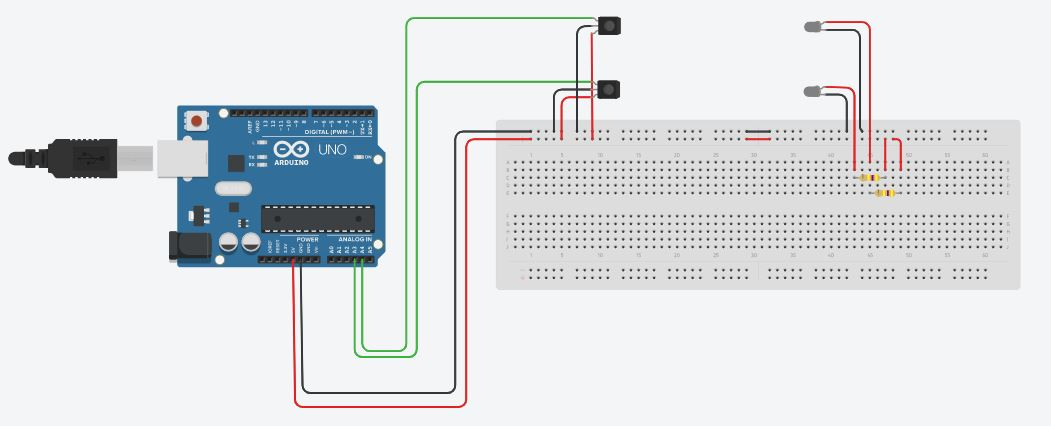
\includegraphics[scale=0.4]{speedometer.png}
	\caption{Circuit diagram of speedometer}
	\end{figure}

\subsection*{Procedure}
\begin{enumerate}[leftmargin=*]
    \item Connect the Arduino microcontroller to the laptop. 
    \item Open Arduino IDE and copy lst. \ref{list:speed} to it.
    \item Measure the distance between the sensors in cm and enter the value in the code (the value currently entered is \textit{float distance =10}). 
    \item Upload your code to the Arduino board.
    \item Once the code is uploaded, open the Serial Monitor.
    \item Take a moving thing, like a ping-pong or a toy car, and pass it from the path cut in the box. The box \textit{must} be placed so that the object passes through the sensor connected to A3 first.
    \item Note the speed registered on the laptop screen. 
    \item Change the speed of the object and repeat the experiment.
\end{enumerate}

\begin{lstlisting}[language=Arduino, numbers=none, caption={Arduino code for measuring the speed of a moving object},captionpos=b, label=list:speed]
int ir1=A3, ir2=A4, val1, val2, pre1, pre2, secondcheck, x, y;
float sped=0;
float distance =10; // Distance between the IR sensors in cm
unsigned long dur, sval, fval;
void setup () {
    // put your setup code here, to run once:
    Serial.begin(9600);
    pinMode(ir1, INPUT);
    pinMode(ir2, INPUT);
    pre1=0;
    pre2=0;
    secondcheck = 0;
    Serial.println(sped) ;
}
void loop (){
    x=analogRead(ir1);
    y=analogRead(ir2);  
    if (x>900)
        val1 = 1;
    else
        val1 = 0;
    if (y>900)
        val2 =1;
    else
        val2 =0;
    if (val1 > pre1)
    {
        sval = millis();
        secondcheck = 1;
    }
    if(val2 > pre2 && secondcheck ==1)
    {
        fval = millis() ;
        dur = fval-sval;
        sped = distance*1000.0/dur;
        secondcheck = 0;
    }
    Serial.print(dur);
    Serial.print(”\ t ”);
    Serial.println(sped);
    pre1 = val1;
    pre2 = val2;
}

\end{lstlisting}

\begin{figure}[H]
\centering
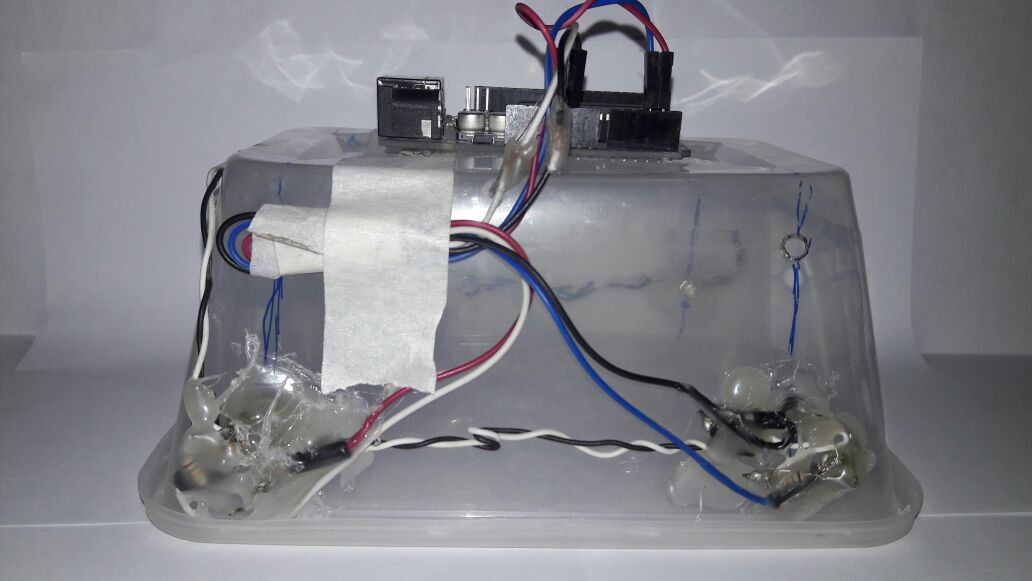
\includegraphics[scale=0.20]{speedometer-hardware-1.jpg}
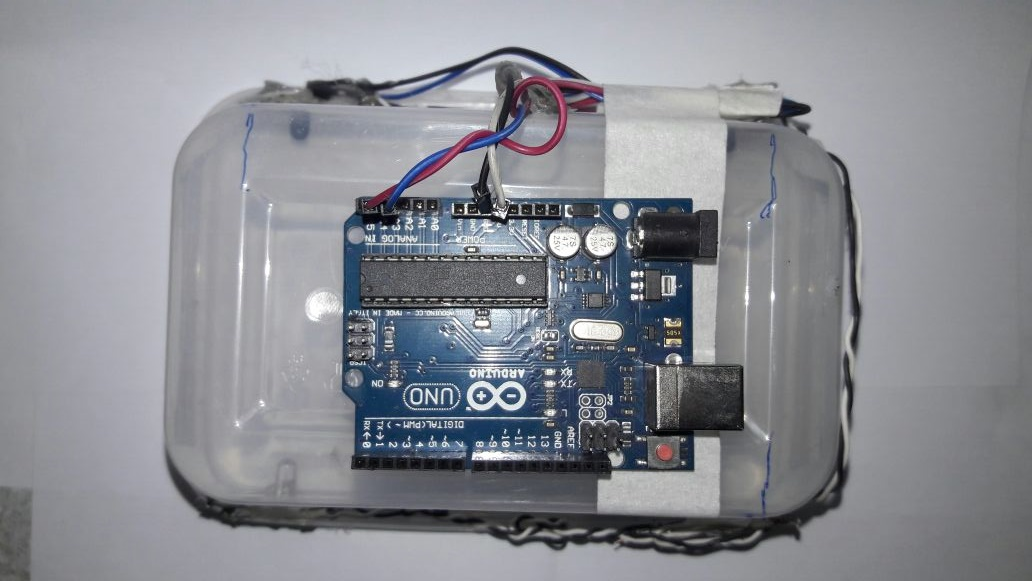
\includegraphics[scale=0.27]{speedometer-hardware-2.jpg}
\caption{Hardware of the speedometer}
\end{figure}